
\paragraph{The ghost in the machine}

In Philip K. Dicks \emph{Do Androids Dream of Electric Sheep?}, which was made into the slightly-more-famed movie \emph{Blade Runner}, the protagonist Deckard works as a policeman specializing in catching runaway and criminal androids. In Deckard's world, AI has advanced to such a level that telling the difference between a machine and a human being takes expert level knowledge.

While Deckard's machines are not the end-all, be-all of AI, they mark the crucial point in coming human history where human beings and machines become indistinguishable to anything but the trained eye.
Imagine we can reach a stage where having a conversation with a machine is no different from having one with a regular human being.
Then, can we say that the machine is not alive?
Can something mechanical be infused with a soul?
Can something consisting of copper wires and transistors, designed in a lab and built in a factory, be just as living as something made of organic materials?
Is it possible that we will \emph{build} life before we discover it?

\begin{center}
	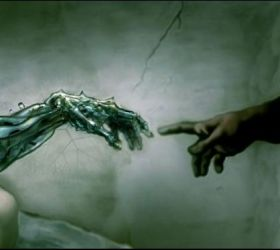
\includegraphics[width=0.475\textwidth]{AI_bilde_four.jpg}
	\tiny{Credit: }
\end{center}

\paragraph{Architects of our own demise}
The subject of science as a force for destruction is a well-known issue.
Engineering has given us the tools to perform miracles, but also the tools to facilitate our own apocalypse.
Recent debates have grown regarding the future dangers of AI.
At its highest ideal, AI will give birth to entities that will seem \emph{god-like} compared to a regular human being.
Future AI will have infinitely higher capacity for information storage and search, instant learning, physical capabilities and endurance vastly superior to our own. We will be powerless to stop them should we make enemies of these machines.
This is the \emph{Terminator} endworld dystopian nightmare, in which human beings are in the process of being exterminated by the superior technology of the machine race. 
AI experts have split opinions on this potential future.
Some believe that these future dangers are negligable; we will always have an element of control, or the machines will have no reason to abuse us.
The benefits of such god-like beings in our employ are beyond imagining.
There is also a line of belief that says humanity will end itself before this kind of AI becomes global.
The very respectable Hugo de Garis presents his theory on \emph{The Artilect War}\cite{artilect}, in which rival factions within the human race will destroy each other before strong AI is made.
The first of these two factions is convinced of the benefits of AI, and wishes to continue to build them, whilst the other is so terrified of the machine future that they make war on the first faction.
With such names as Stephen Hawking and Elon Musk (whom, in fairness, are not AI experts) speaking out against the development of AI, a careful eye has to be kept on the development of these technologies.